% -*-latex-*-
\documentclass[handout]{beamer}
%\documentclass[12pt]{beamer}
\usepackage{etex,graphicx,moreverb}
\usepackage{wasysym}
\usepackage{amsmath}
\usepackage{graphicx}

\let\latexput\put
\usepackage{pictex}
\let\pictexput\put
\let\put\latexput

\title{Alleles and Genotypes in Populations that Mate at Random}
\author{Alan R. Rogers}
\date{\today}
%\setbeamercovered{transparent}
\begin{document}

\frame{\titlepage}

\begin{frame}
\frametitle{Three systems of vocabulary}
\begin{tabular}{p{2.2in}ccc}
                        &   1   & 2 & 3\\
Position on chromosome  & locus & locus & locus\\
Protein-coding locus    & gene  & gene & gene\\
Physical copy of DNA at locus  & gene  & allele &gene copy\\
One of several variants at a locus& allele & allele & allele\\
\end{tabular}

\bigskip

1 is classical usage, 2 is Gillespie's, and we try to keep to 3.
\end{frame}

\begin{frame}
\frametitle{Illustration of classical usage}
Those organisms (homozygotes) which received like genes, in any pair
of corresponding loci, from their two parents, would necessarily hand
on genes of this kind to all of their offspring alike; whereas those
(heterozygotes) which received from their two parents genes of
different kinds\ldots (Fisher, 1930, p.~8)
\end{frame}

\begin{frame}
  \frametitle{The same sentence in the three systems}
  \begin{description}
    \item[Classical] If the \emph{genes} you inherited from mom and dad are
      different alleles, then you are a heterozygote.
    \item[Gillespie] If the \emph{alleles} you inherited from mom
      and dad are different alleles, then you are a heterozygote.
    \item[Us] If the \emph{gene copies} you inherited from mom and dad are
      different alleles, then you are a heterozygote.
  \end{description}
  
\end{frame}

\begin{frame}
\frametitle{Transferrin genotype frequencies in a baboon troop}
\begin{columns}
\column{0.5\textwidth}
\begin{tabular}{rrrr}
        &\multicolumn{3}{c}{Number of}\\ \cline{2-4}
G'type& baboons &$C$&$D$\\ \hline
$CC$    &  80 & 160&  0\\
$CD$    &  15 &  15& 15\\
$DD$    &   5 &   0& 10\\ \hline
Total   & 100 & 175& 25\\
\end{tabular}
\column{0.5\textwidth}
\begin{tabular}{r@{$\;=\;$}c@{$\;=\;$}l}
\multicolumn{3}{c}{Relative frequency}\\ \hline
$\hat x_{CC}$&80/100&0.80\\
$\hat x_{CD}$&15/100&0.15\\
$\hat x_{DD}$& 5/100&0.05\\
$\hat p$ & 175/200 & 0.875
\end{tabular}
\end{columns}

\bigskip
Note: ``hat'' indicates values describing sample rather than
population. I'll often ignore this distinction.
\end{frame}

\begin{frame}
\frametitle{Alternative calculation of $p$}
\begin{eqnarray*}
\hat p &=& \hat x_{CC} + \hat x_{CD}/2\\
&=& 0.80 + 0.15/2 = 0.875
\end{eqnarray*}
The sample allele frequency $\hat p$ is an estimate of the population allele
frequency $p$.

\bigskip

The population allele frequency is also the probability that a gene drawn at
random from the population is a copy of allele~$C$.
\end{frame}

\begin{frame}
\frametitle{Allele frequency as probability}
Suppose there are two alleles, $A_1$ and $A_2$, with frequencies $p$
and $1-p$. What is the probability that a random gene copy is an
$A_1$? 

\bigskip
\pause

It is just the relative frequency, $p$, of a allele $A_1$ within the population.

\bigskip
\pause

You can also think of it this way: select a random individual, and
from that individual choose a random gene. You end up with $A_1$ with
probability 
\[
p = P_{11}\times 1 + P_{12}\times\frac{1}{2}
\]
where $P_{11}$ and $P_{12}$ are the frequencies of genotypes $A_1A_1$
and $A_1A_2$.
\end{frame}

\begin{frame}
\frametitle{Expected genotype frequencies}

What is the probability that a random baboon will have genotype $CD$?

\bigskip
\pause

If we know the genotype frequencies, the answer is $x_{CD}$, the
genotype frequency.

\bigskip
But what if we only know the allele frequency?

\bigskip
\pause

Then the answer depends on characteristics of population.  To
describe these effects, we need a model.
\end{frame}

\begin{frame}
\includegraphics[width=\linewidth]{hwequil.png}
\end{frame}

\begin{frame}
\frametitle{Model: random mating, no selection}

Event $CD$ can be decomposed as follows:
\begin{center}
\begin{tabular}{ccll}
\multicolumn{2}{c}{Gene copy from}\\ \cline{1-2}
Mom  & Dad & Probability\\
\cline{1-3}
$C$  & $D$ & $p \times (1-p)$ & \hspace{2em}Why multiply?\\
$D$  & $C$ & $(1-p) \times p$ & \hspace{2em}Why multiply?\\
\cline{1-3}
\multicolumn{2}{c}{Sum:} & $2p(1-p)$ & \hspace{2em}Why add?
\end{tabular}
\end{center}
\end{frame}

\begin{frame}
\frametitle{Event $CC$}
\begin{center}
\begin{tabular}{ccll}
\multicolumn{2}{c}{Gene copy from}\\ \cline{1-2}
Mom  & Dad & Probability\\
\cline{1-3}
$C$  & $C$ & $p \times p$ & Why multiply?\\
\cline{1-3}
\multicolumn{2}{c}{Sum:} & $p^2$
\end{tabular}
\end{center}
\end{frame}

\begin{frame}
\frametitle{Hardy-Weinberg result}
\begin{center}
\begin{tabular}{cc}
  & Relative\\
Genotype & frequency\\ \hline
$CC$ & $x_{CC} = p^2$\\
$CD$ & $x_{CD} = 2pq$\\
$DD$ & $x_{DD} = q^2$\\\hline
\multicolumn{2}{c}{\rule{0pt}{2.5ex}Where $q=1-p$.}
\end{tabular}
\end{center}
\begin{itemize}
\item Random mating does not change $p$.
\item Given allele frequency, we can predict genotype frequencies.
\end{itemize}
\pause This assumes an infinite population with random mating and no
selection. Real populations aren't like that, so why should we care
about Hardy-Weinberg?
\end{frame}

\begin{frame}
\frametitle{Observed versus expected g'type freqs}
\begin{center}
  \begin{tabular}{ccc}
        & \multicolumn{2}{c}{Relative frequency}\\ \cline{2-3}
Genotype& Observed & Expected\\ \hline
$CC$ &$x_{CC} = 0.80$ & $p^2 = 0.77$\\
$CD$ &$x_{CD} = 0.15$ & $2pq = 0.22$\\
$DD$ &$x_{DD} = 0.05$ & $q^2=0.02$\\ \hline
\end{tabular}
\end{center}
Observed: relatative frequency of genotype in data\\
Expected: Hardy-Weinberg formula
\end{frame}

\begin{frame}
\frametitle{Heterozygosity on human chromosome~1}
\centering
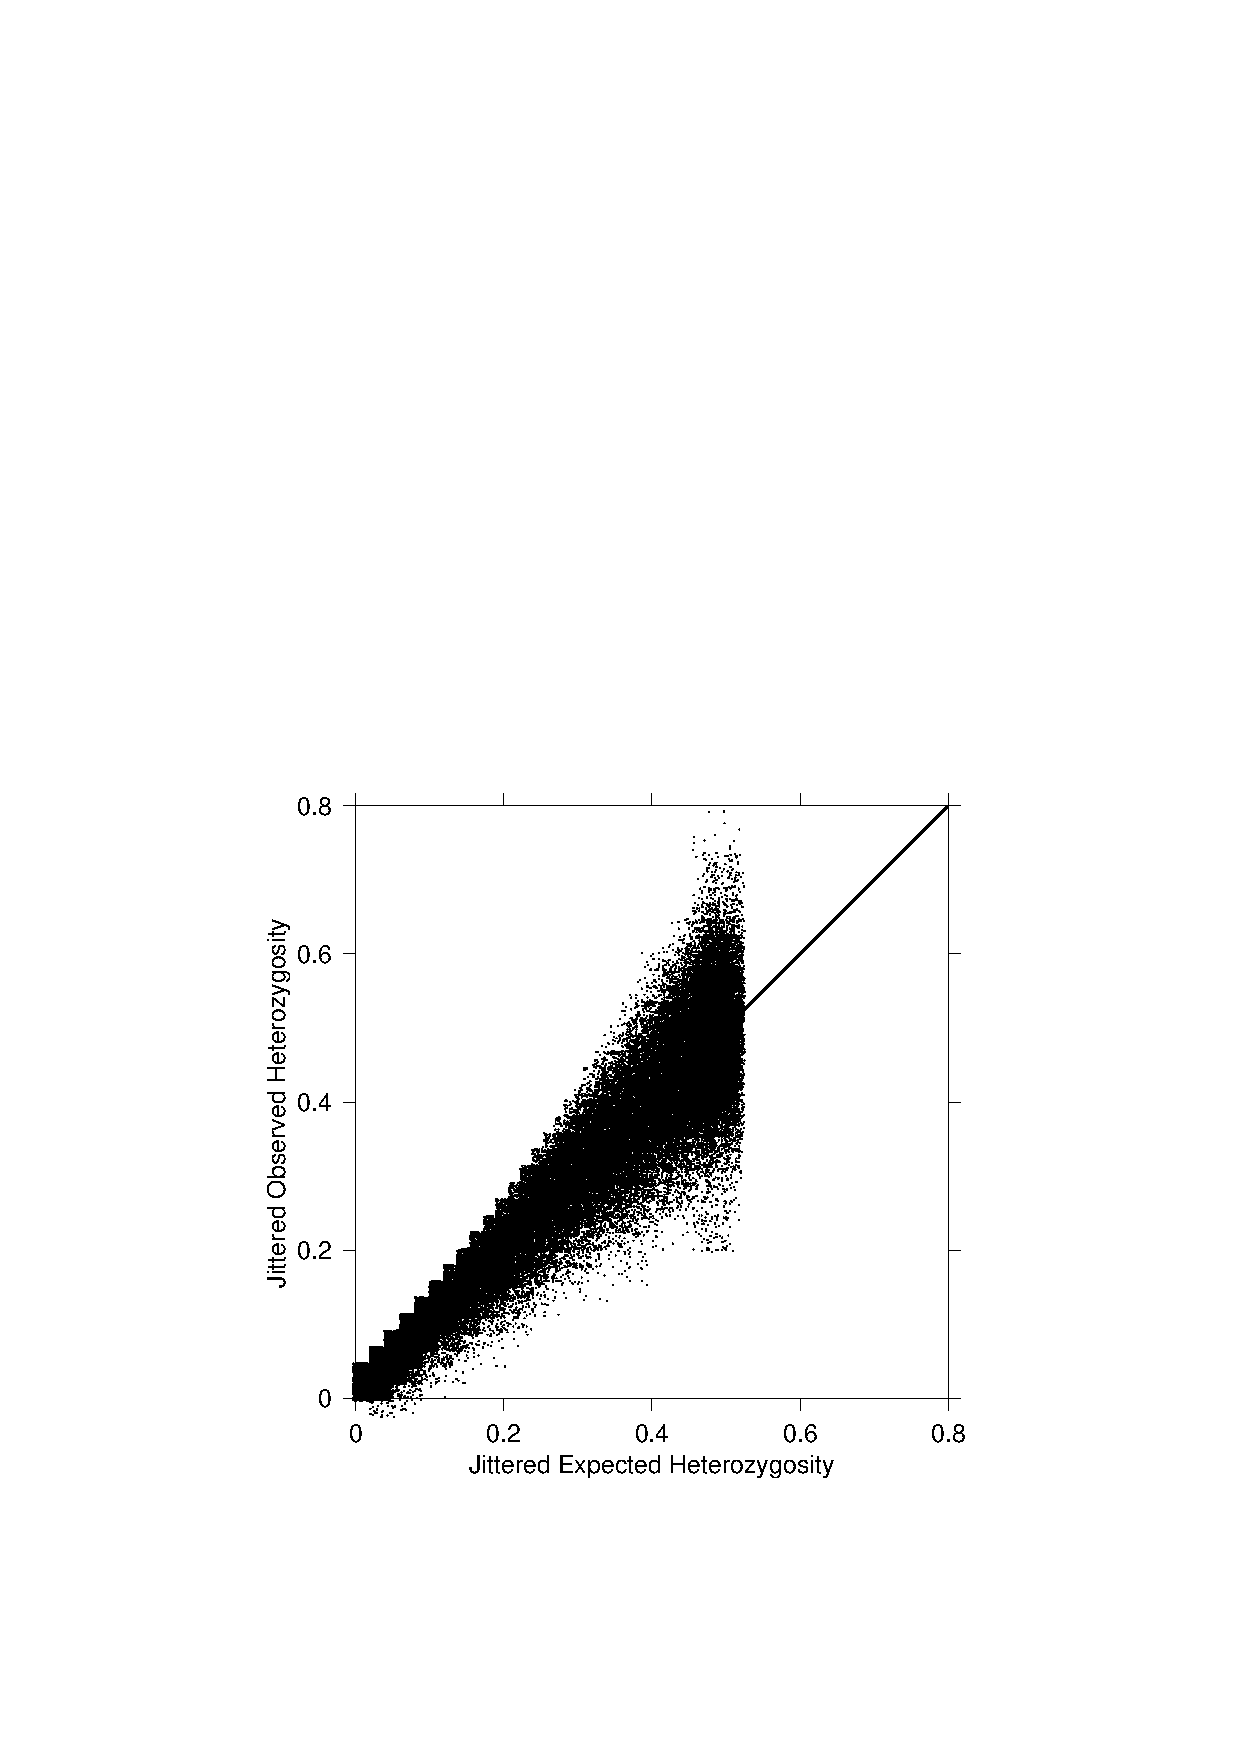
\includegraphics[width=0.78\textwidth]{hweq.png}\\
\end{frame}

\begin{frame}
\frametitle{What if males and females have different allele
  frequencies?}
{\centering
\begin{tabular}{cccc}
 & \multicolumn{3}{c}{Genotype frequencies}\\ \cline{2-4}
Sex   & $A_1A_1$ & $A_1A_0$ & $A_0A_0$\\
\hline
\male & $x_{11}$    & $x_{10}$    & $x_{00}$\\
\female & $y_{11}$  & $y_{10}$    & $y_{00}$
\end{tabular}\\[2ex]

\onslide<2->{%
\begin{tabular}{cl}
Sex & Allele frequency\\
\hline
\male & $p_m = x_{11} + x_{10}/2$\\
\female & $p_f = y_{11} + y_{10}/2$
\end{tabular}\\}}
\end{frame}

\begin{frame}
\frametitle{An autosomal locus in a nuclear family}
\begin{columns}
\column{0.4\textwidth}
{\centering\let\put\pictexput
\mbox{\beginpicture
\setcoordinatesystem units <1cm,1cm>
\setplotarea x from 0 to 4, y from 0 to 4
%\axis left ticks andacross numbered from 0 to 4 by 1 /
%\axis bottom ticks andacross numbered from 0 to 4 by 1 /
\put {\makebox(0,0)[b]{Dad}} at 1 3.6
\put {\makebox(0,0)[b]{Mom}} at 3 3.6
\put {\makebox(0,0)[t]{Child}} at 2 0.4
\put {$\bullet$} at 0.8 3
\put {$\bullet$} at 1.2 3
\put {$\bullet$} at 2.8 3
\put {$\bullet$} at 3.2 3
\put {$\bullet$} at 1.8 1
\put {$\bullet$} at 2.2 1
\put {?} [tr] <-1pt,0pt> at 1.45 2.1
\put {?} [tl] <1pt,0pt> at 2.55 2.1
\arrow <8pt> [0.2,0.67] from 1.2236 2.5528 to 1.7764 1.4472
\arrow <8pt> [0.2,0.67] from 2.7764 2.5528 to 2.2236 1.4472
\circulararc 360 degrees from 1.5 3 center at 1 3
\circulararc 360 degrees from 3.5 3 center at 3 3
\circulararc 360 degrees from 2.5 1 center at 2 1
\endpicture}
\let\put\latexput
\\}
\column{0.6\textwidth}
\onslide<2->{%
Probabilities that gametes carry $A_1$\\[1ex]
{\centering\begin{tabular}{cl}
\male & $x_{11} + x_{10}/2 \onslide<3->{= p_m}$\\
\female & $y_{11} + y_{10}/2 \onslide<3->{= p_f}$\\
\end{tabular}\\}}

\bigskip

\pause
\onslide<4->{%
Child genotype probabilities
\begin{align*}
x'_{11} &= p_m p_f\\
x'_{10} &=  p_m (1-p_f) + p_f(1-p_m)\\
x'_{00} &=  (1-p_m)(1-p_f)
\end{align*}}
\end{columns}

\bigskip

\onslide<5->{\rule{\textwidth}{0.4pt}
 After one generation of random mating, the sexes have equal
 allele frequencies at autosomal loci.
\begin{align*}
p' &= x'_{11} + x'_{10}/2\\
 &= (p_m + p_f)/2
\end{align*}}
\end{frame}

\begin{frame}
\frametitle{Summary}
\begin{itemize}
\item At equilibrium under random mating, allele frequencies determine
  genotype frequencies.
\item Hermaphrodites reaches equilibrium in 1 generation.
\item Autosomal loci in sexual populations reach equilibrium in 2
  generations.
\item X-linked loci in reach equilibrium only gradually.
\end{itemize}
\end{frame}

\end{document}
